\documentclass[a4paper,twoside]{article}
\usepackage[small]{caption}
\usepackage{epsfig}
%\usepackage{subfigure}
\usepackage[subrefformat=parens,labelformat=parens]{subfig}
\usepackage{graphicx}
\usepackage{calc}
\usepackage{amssymb}
\usepackage{amstext}
\usepackage{amsmath}
\usepackage{amsthm}
\usepackage{multicol}
\usepackage{pslatex}
\usepackage{apalike}
\usepackage{SCITEPRESS}
\usepackage{mathrsfs}
\captionsetup[subfloat]{farskip=0pt,nearskip=0pt,captionskip=5pt}


%\subfigtopskip=0pt
%\subfigcapskip=0pt
%\subfigbottomskip=0pt

\begin{document}

\title{Homotopy Surface Cutting Using Edges' Sources in Geodesic Distance}

\author{\authorname{Anuwat Dechvijankit,Author2 and Author3}
\affiliation{Department of Computational Intelligence and Systems Science, Tokyo Institute of Technology, Japan}
\email{dechvijankit.a.aa@m.titech.ac.jp}
}

\keywords{geodesic distance, graph cut, homotopy, surface parameterization}


\abstract{Topology is a property in surfaces that plays a major role in computer graphics. Processing or analysis between two surfaces generally requires both of them to be same topology. There are many tools or applications such as parameterization or remeshing that require disk topology surfaces as input. Therefore, we need convert any surfaces to be same as a topological disk. The common procedure is to define a graph of edges inside the surface that should be split into two edges and to turn the surface into topological disk. We call it as homotopy cutting. Problems become more difficult when dealing with high genus surfaces such as a torus. Based on a novel method, we present an enhancement method to generate a cut graph in high-genus surface for homotopy cutting. By using geodesic properties of each edge, we can generate equally or more suitable edge-graph than original method while remaining performance and stability as original one.}

\onecolumn \maketitle \normalsize \vfill

\section{\uppercase{Introduction}}
\label{sec:introduction}

\noindent Geometry processing is an important research in 3D computer graphics field. Without efficient algorithms, it is very difficult to develop any kinds of advanced application for end-users. Some of important applications in 3D computer graphics, such as texture mapping \cite{Bennis:1991:PSF:127719.122744}, normal mapping \cite{Cohen:1998:AS:280814.280832}, remeshing \cite{Hormann00quadrilateralremeshing} and parameterization \cite{Tutte:1963,Floater:1997:PSA:248299.248308} require specific topology of input mesh. There are many cases where topological disk surface is specified for further processing. Such topological requirement in input mesh has significant impact on several researches. There are many properties in each mesh such as closed/open, holes and genus: which affect to selection of measurement.

When dealing with a mesh that requires disk topology input, all kinds of meshes have different measures. Open surface has originally the same topology as disk which can pass directly but may need to be taken care in case of containing holes. The problems arise when dealing with closed surface since it has different topology from disk. The process to cutting surface into the disk is required. In case of sphere topology, it does not require much processes; only short graph edge is necessary. However, there is some processes to ensure quality that require more graph edges in homotopy cutting. The problem becomes more complex and more interesting when dealing with high genus surfaces. 
   
This paper presents a homotopy cutting on high genus surfaces. Our approach is an enhancement of a novel method \cite{Gu:2002:GI:566654.566589} in homotopy cutting; cutting surface into disk. A benefit of this method is to able to handle any kinds of 2-manifold surfaces, regardless of specific topology. We present an algorithm that creates a cut graph on the area where geodesic path comes from different directions in exact geodesic distance \cite{Mitchell:1987:DGP:33367.33372,Surazhsky:2005:FEA:1073204.1073228} (see example in figure \ref{fig:geodesic rocket arm}). With an few extra calculation,  we can define equally or more appropriate cut graph from original method while remaining performance and stability.
\begin{figure}[!h]
	\centering
	{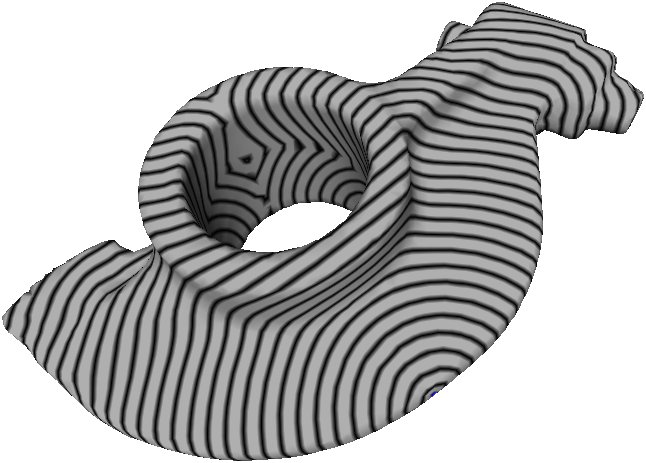
\includegraphics[width=0.9\columnwidth]{images/geodesic_rocket-arm.png}}
	\caption{Geodesic distance radius from a starting point on genus 1 rocket arm model. At the hole, we can see some sharp pattern which can be recognize as geodesic path came from different directions.}
	\label{fig:geodesic rocket arm}
\end{figure}

\subsection{Notations}
Before explaining various algorithms of homotopy, let us define basic notations. We represent a 2-manifold triangular surface or mesh by $\mathscr{M}:=(V,F)$, where $V:=\{ v_{i}\in \mathbb{R}^3 \mid i = 1, ... , n_v\}$ is a set of $n_v$ vertices and $F:=\{ f_{i}(a,b,c) \mid a,b,c = 1, ... , n_v : a \neq b \neq c\}$ is a set of $n_f$ faces. We also define $E:=\{ e_{i}(a,b) \mid a,b = 1, ... , n_v : a \neq b\}$ as a set of $n_e$ edges found in the surface $\mathscr{M}$. We assume that the mesh has genus $g$ topology. 


\section{\uppercase{Related Works}}
\label{sec:related works}
\noindent As for a topic of topological converting topic in the past years, there was a novel work  by \cite{Erickson:2002:OCS:513400.513430} that studied the problem of cutting a topological surface into the disk efficiently. They have proposed a cutting method that has some elegant theoretical guarantees but is complex to implement. It finds the shortest loop path connecting a vertex to the vertex itself by using a front propagation technique, and then tests to see if the considering loop path reduces the surface genus or simply cut the surface into two pieces. It has topologically-sufficient cut as $2g$ loops. The generation of minimal length cuts that convert a high genus surface into a topological disk is a NP-hard problem. One method is a brute force approach which consumes a lot of time. However, it is an approximation of the shortest cut graph in $O(g^2 n \log n)$ where $n$ denotes complexity of the surface. \cite{Erickson:2005:GOH:1070432.1070581} studied about a greedy homotopy basis and improved its calculation speed in $O(n \log n)$
by using a straightforward application of Dijkstra's shortest path algorithm \cite{Dijkstra59anote}. 

From the efficiency point of view, it is important to compute non-trivial cycles on orientable surfaces. Non-trivial cycles mean non-contractible and non-separating cycles which guarantees cutting topological surface into disk. Recently, \cite{Kutz:2006:CSN:1137856.1137919} presents an algorithm that computes a shortest non-trivial cycle in $O(n \log n)$ on orientable combinatorial surface of bounded genus. The algorithm is based on universal-cover constructions to find short cycles.

There are several studies trying to define a cut graph by surface properties. Study by \cite{Patane:2007:FCB:1224804.1224947} presents an algorithm that builds up the cut graph on the iso-contours from Reeb graph which codes the topology of a given surface $\mathscr{M}$ in a combinatorial structure and generates loops together. Another study by \cite{Jin:2013:CSH:2396897.2396971}, presents an algorithm to compute the shortest homotopic loop with negative Euler characteristic based on the surface hyperbolic uniformization metric. They also demonstrate two applications: constructing extremal quasi-conformal mappings between same topology surfaces, and detecting homotopy between two paths or cycles on a surface. 

There is an iterative method called "geometry images" by \cite{Gu:2002:GI:566654.566589}. This method presents a remeshing approach using square surface parameterization to create irregular surface $\mathscr{M}$ in $\mathbb{R}^3$ domain, square planar in $\mathbb{R}^2$ domain and sample positions to get a regular positions. To get low error on remeshing, they present how to create a cut graph from any kinds of surface $\mathscr{M}$ regardless from the pre-analysis of topology and boundary edges.

\begin{figure}[!h]
	%\vspace{-0.2cm}
	\centering
	\subfloat[Geometry of surface]{\label{fig:gim3d}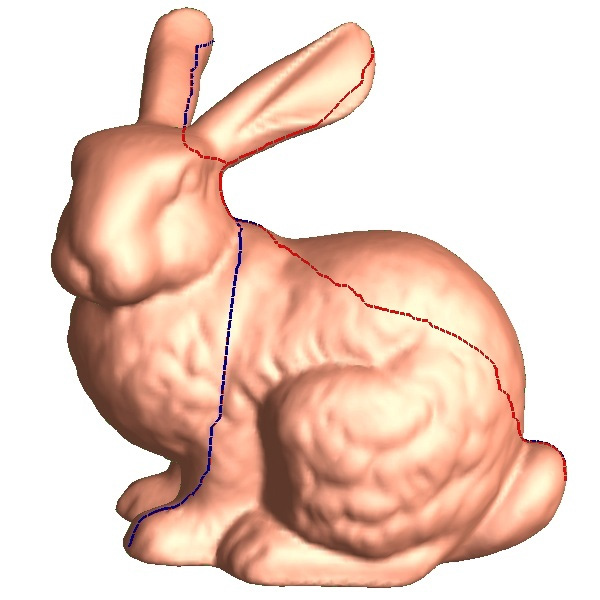
\includegraphics[width=0.45\columnwidth]{images/gim_bunny3D.png}}
	\subfloat[Geometry image]{\label{fig:gim2d}
\includegraphics[width=0.45\columnwidth]{images/gim_bunny2D.png}}
	
	\caption{A geometry image.}
	\label{fig:gim figure}
\end{figure}

Since our approach is based on geometry images, in section \ref{sec:previous algorithm}, we explain how it creates a cut graph for homotopy cutting on irregular surface $\mathscr{M}$ with genus $g$.
\section{\uppercase{Previous Algorithm}}
\label{sec:previous algorithm}
\noindent The algorithm of \cite{Gu:2002:GI:566654.566589} is divided into two parts, homotopy cutting and its augmentation. The augmentation aims to improve subsequent square planar domain parameterization. We explain the first part that involves the definition of a cut graph and a converting surface $\mathscr{M}$ into disk.

\begin{figure*}[t]
	\centering		
	\subfloat[\label{fig:OriginalGenusReduceMethodStepByStep-a}]{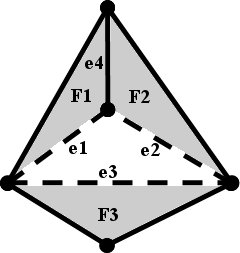
\includegraphics[width=0.400\columnwidth]{images/fig-original_genus_reduce_method_step_by_step-a.png}}\hspace{10pt}
	\hspace{0.000\columnwidth}
	\subfloat[\label{fig:OriginalGenusReduceMethodStepByStep-b}]{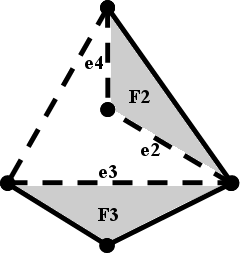
\includegraphics[width=0.400\columnwidth]{images/fig-original_genus_reduce_method_step_by_step-b.png}}\hspace{10pt}		
	\hspace{0.000\columnwidth}
	\subfloat[\label{fig:OriginalGenusReduceMethodStepByStep-c}]{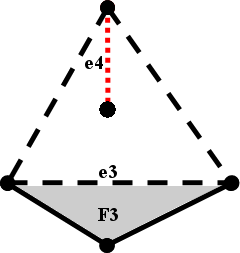
\includegraphics[width=0.400\columnwidth]{images/fig-original_genus_reduce_method_step_by_step-c.png}}\hspace{10pt}		
	\hspace{0.000\columnwidth}
	\subfloat[\label{fig:OriginalGenusReduceMethodStepByStep-d}]{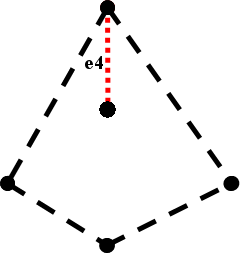
\includegraphics[width=0.400\columnwidth]{images/fig-original_genus_reduce_method_step_by_step-d.png}}		
	\caption{Processes after removing a seed triangle from mesh. Gray areas mean that there are still triangles, while white areas mean triangles have been removed. Dash lines mean edges that are adjacent to only one triangle at the moment. \subref{fig:OriginalGenusReduceMethodStepByStep-a} shows the moment after removing the seed triangle; that is, edges e1,e2 and e3 are only edges that are adjacent to only one triangle. Assume that edge e1 has the smallest geodesic distance from the seed triangle at the moment. \subref{fig:OriginalGenusReduceMethodStepByStep-b} shows the result of removing edge e1 and face F1 according to the condition. At this moment, edge e4 is also adjacent to only one triangle same as edge e2. Let e2 have smaller geodesic distance than edges e3 and e4.  \subref{fig:OriginalGenusReduceMethodStepByStep-c} shows the result of removing edge e2 and face F2 without removing edge e4. Because of the edge e4 is not adjacent any triangle after removing face F2, it is excluded from adjacent only one triangle's condition. The edge e4 becomes a candidate of seam-cutting edge. \subref{fig:OriginalGenusReduceMethodStepByStep-d} shows the result of next step from \subref{fig:OriginalGenusReduceMethodStepByStep-c} that removing triangle F3 and edge e3. (TO DO: change images)}
	\label{fig:OriginalGenusReduceMethodStepByStep}
\end{figure*}

At the beginning in the method , if the mesh has boundaries, let $\mathscr{B}$  be the set of original boundary edges that remain unchanged in the whole process and will be included in final cut graph ${\rho}$. It first starts by removing a single seed triangle from the mesh. At this moment, each edge of the seed triangle is adjacent to only one triangle respectively (see figure \subref*{fig:OriginalGenusReduceMethodStepByStep-a}).  After removing the seed triangle from the mesh, there are two phases of processing.

In the first phase, it repeatedly detects an edge adjacent exactly to one triangle that is not in $\mathscr{B}$, and removes both the edge and the triangle from the mesh structure. The rest two edges are left (see figure \subref*{fig:OriginalGenusReduceMethodStepByStep-b}). If the rest edges of the removing triangle are not adjacent to any triangle, then the edges will become one of candidates of cut graph (see figure \subref*{fig:OriginalGenusReduceMethodStepByStep-c}). Generally, removing one edge and one triangle triggers more two edges to be adjacent to only one triangle further. Considering the mentioned condition, the removing propagation will keep spreading out from the seed triangle according to geodesic distance in order to get minimum radius result (see figure \subref*{fig:OriginalGenusReduceMethodStepByStep-d}). Since a 2-manifold triangle mesh is being processed, any triangle will be removed eventually. Therefore, this phase ends when there is no triangle left and there remain only edges and their vertices as candidate cut graph edges (see figure \subref*{fig:fig-original_genus_reducing_process-c}). At this point, the cut $\rho$ consists of a set of connecting $2g$ loops.

In the second phase, we again iteratively detect a valence-1 vertex and its corresponding edge, and remove both the vertex and the edge (see figure \ref{fig:fig-original_remove_dangling_edges_step_by_step}). The purpose of this phase is to remove unnecessary dangling edges in the first phase. The dangling edges will be repeatedly trimmed away until there is no valence-1 vertex in the cut $\rho$ left. There are only edges that form connected loops as a cut graph in the cut $\rho$. At Last, all loops in $\rho$ are straightened by computing a local shortest path in each loop. Finally, the connected $2g$ loop cut graph in $\rho$ is homotopy basis: a cut graph that convert surface into a topological disk patch. See figure \ref{fig:fig-original_genus_reducing_process} for overall process of finding graph cut on a genus-3 mesh.


\begin{figure}[bh!]
	\centering		
	\subfloat[\label{fig:fig-original_remove_dangling_edges_step_by_step-a}]{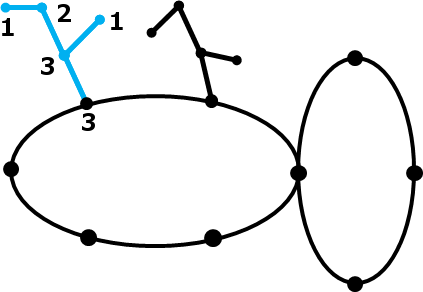
\includegraphics[width=0.40\columnwidth]{images/fig-original_remove_dangling_edges_step_by_step-a.png}} \hspace{10pt}
	\subfloat[\label{fig:fig-original_remove_dangling_edges_step_by_step-b}]{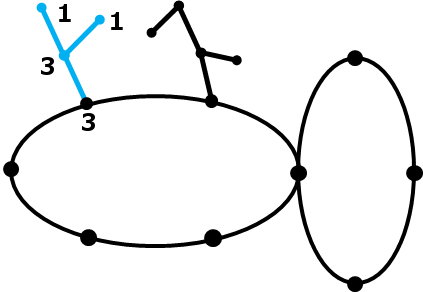
\includegraphics[width=0.40\columnwidth]{images/fig-original_remove_dangling_edges_step_by_step-b.png}}\\		
	\subfloat[\label{fig:fig-original_remove_dangling_edges_step_by_step-c}]{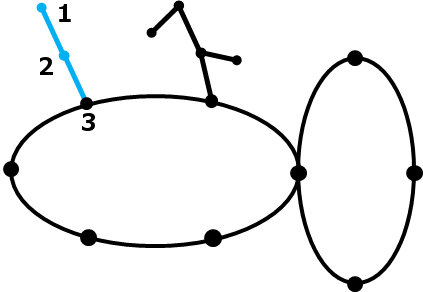
\includegraphics[width=0.40\columnwidth]{images/fig-original_remove_dangling_edges_step_by_step-c.png}}	\hspace{10pt}	
	\subfloat[\label{fig:fig-original_remove_dangling_edges_step_by_step-d}]{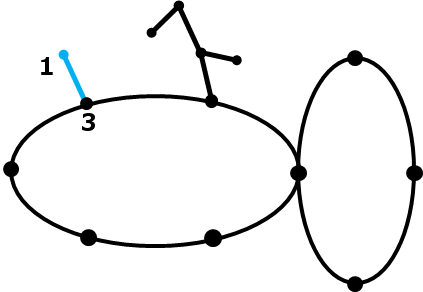
\includegraphics[width=0.40\columnwidth]{images/fig-original_remove_dangling_edges_step_by_step-d.png}}	\\
	\subfloat[\label{fig:fig-original_remove_dangling_edges_step_by_step-e}]{
\includegraphics[width=0.40\columnwidth]{images/fig-original_remove_dangling_edges_step_by_step-e.png}}	\hspace{10pt}
	\subfloat[\label{fig:fig-original_remove_dangling_edges_step_by_step-f}]{
\includegraphics[width=0.40\columnwidth]{images/fig-original_remove_dangling_edges_step_by_step-f.png}}	 
	\caption[]{Process on removing dangling edges. Numbers on vertices indicate present valence number. We focus on the removing of blue dangling edges. \subref{fig:fig-original_remove_dangling_edges_step_by_step-a} shows initial state where there are two valence-1 edges in blue dangling edges at the moment. \subref{fig:fig-original_remove_dangling_edges_step_by_step-b} shows the next step from \subref{fig:fig-original_remove_dangling_edges_step_by_step-a} that removes one of valence-1 edge along with its vertex. The order of removing is not important. \subref{fig:fig-original_remove_dangling_edges_step_by_step-c} and \subref{fig:fig-original_remove_dangling_edges_step_by_step-d} show iteration process of removing valence-1 edge and vertex on blue dangling edges. \subref{fig:fig-original_remove_dangling_edges_step_by_step-e} shows that all blue dangling edges have been removed. \subref{fig:fig-original_remove_dangling_edges_step_by_step-f} shows the process of removing other dangling edges until valence-1 edge has not been found.}
	\label{fig:fig-original_remove_dangling_edges_step_by_step}
\end{figure}
For the case of closed surface of genus 0, the overall processes from this part will generate the cut $\rho$ that consists of only one vertex. To be able to map into planar domain, we add two adjacent edges of the vertex into the cut graph $\rho$. On the other hand, for the case of a mesh having one or more holes, it will result in connected graphs between any two holes.
\begin{figure}[h!]
	\centering		
	\subfloat[\label{fig:fig-original_genus_reducing_process-a}]{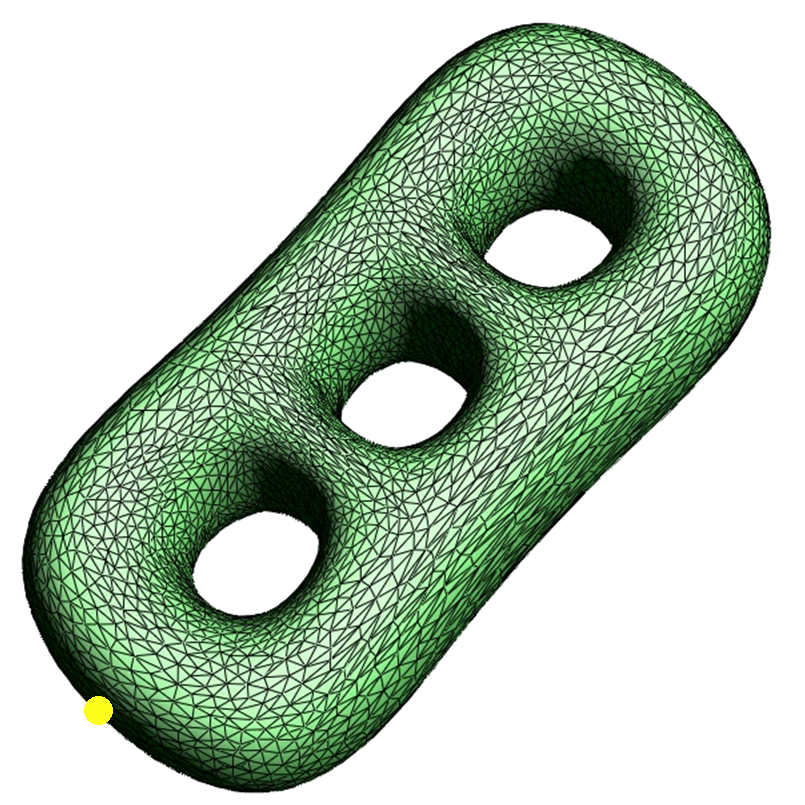
\includegraphics[width=0.31\columnwidth]{images/fig-original_genus_reducing_process-a.png}}
	\hspace{0.00\columnwidth}
	\subfloat[\label{fig:fig-original_genus_reducing_process-b}]{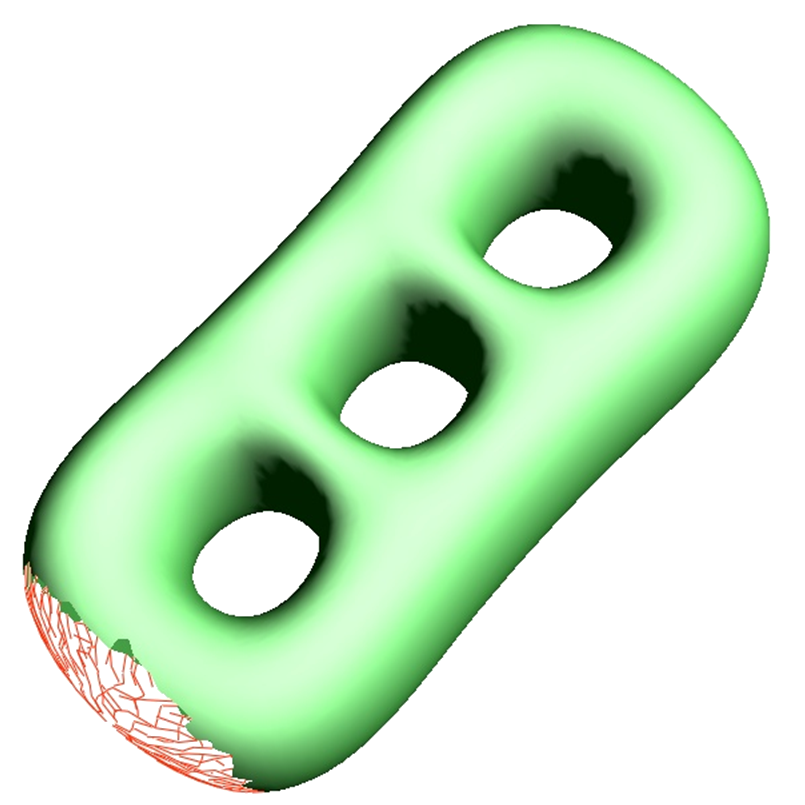
\includegraphics[width=0.31\columnwidth]{images/fig-original_genus_reducing_process-b.png}}
	\hspace{0.00\columnwidth}
	\subfloat[\label{fig:fig-original_genus_reducing_process-c}]{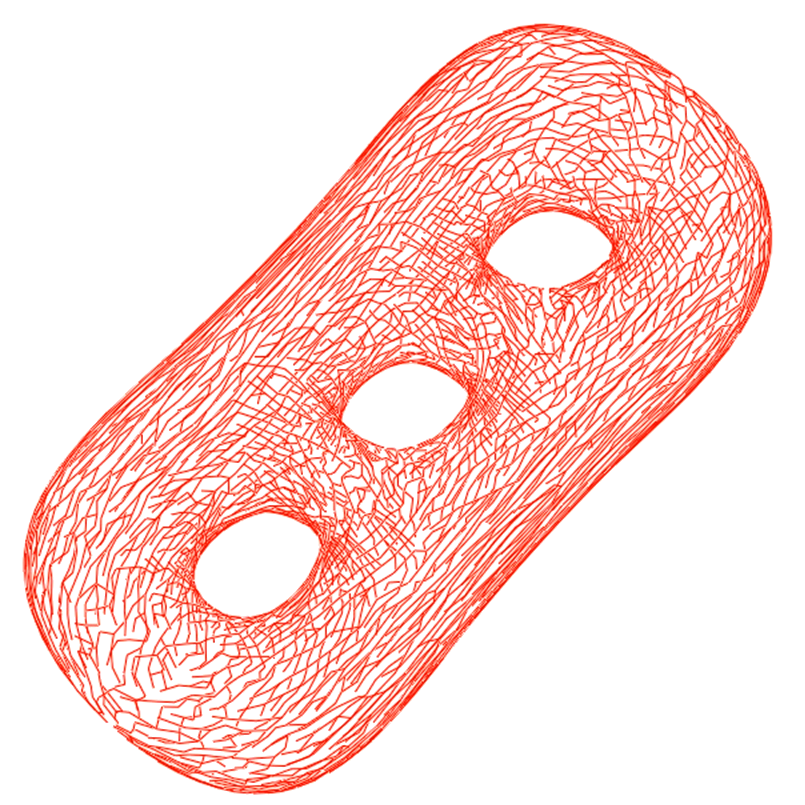
\includegraphics[width=0.31\columnwidth]{images/fig-original_genus_reducing_process-c.png}}
	\hspace{0.00\columnwidth}
	\subfloat[\label{fig:fig-original_genus_reducing_process-d}]{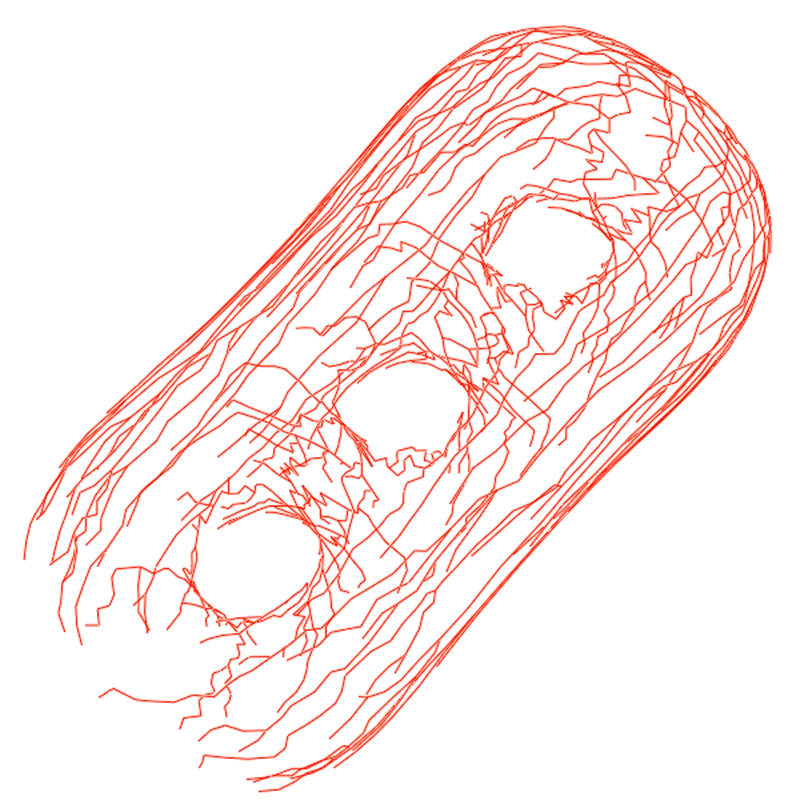
\includegraphics[width=0.31\columnwidth]{images/fig-original_genus_reducing_process-d.png}}
	\hspace{0.00\columnwidth}
	\subfloat[\label{fig:fig-original_genus_reducing_process-e}]{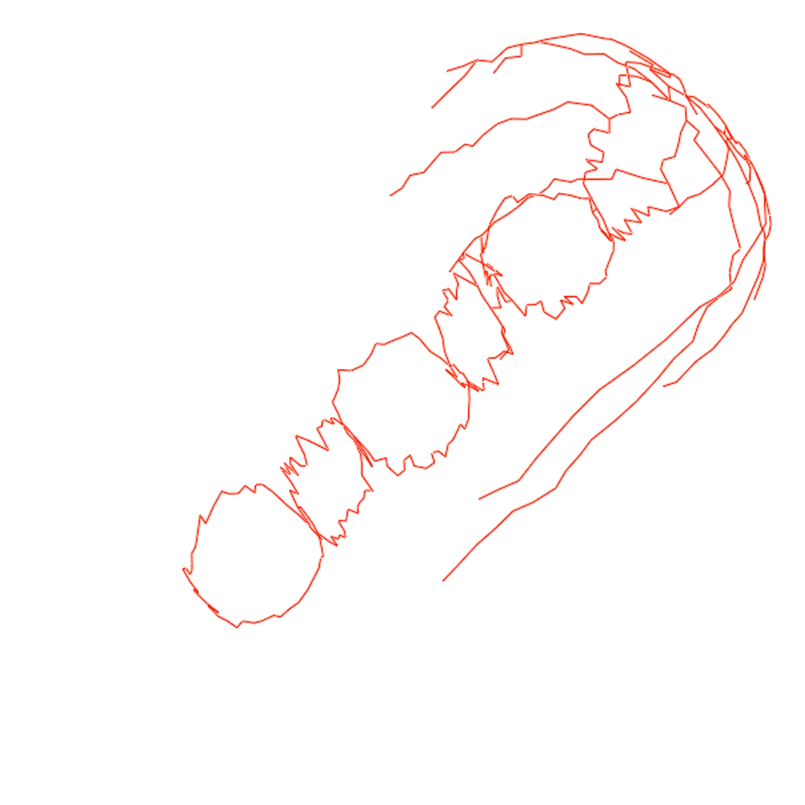
\includegraphics[width=0.31\columnwidth]{images/fig-original_genus_reducing_process-e.png}}
	\hspace{0.00\columnwidth}
	\subfloat[\label{fig:fig-original_genus_reducing_process-f}]{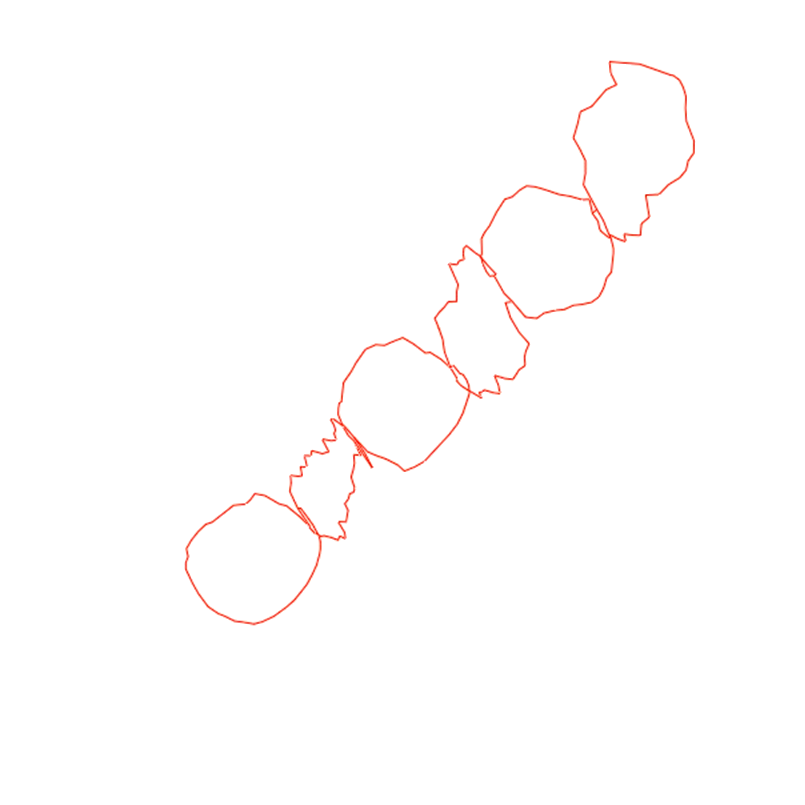
\includegraphics[width=0.31\columnwidth]{images/fig-original_genus_reducing_process-f.png}}
	\caption[]{Process of genus-reduce cutting by sequentially removing triangles, edges and vertices. \subref{fig:fig-original_genus_reducing_process-a} shows a closed genus-3 mesh with one seed triangle (yellow dot). \subref{fig:fig-original_genus_reducing_process-b} shows the intermediate state of mesh when removing triangles and edges that are adjacent to only one triangle. \subref{fig:fig-original_genus_reducing_process-c} shows edge skeleton mesh after removing all triangles. \subref{fig:fig-original_genus_reducing_process-d} and \subref{fig:fig-original_genus_reducing_process-e} show the intermediate state of mesh when removing edges and vertices that are adjacent to only one edge. \subref{fig:fig-original_genus_reducing_process-f} shows final result of straightened cutting edges after removing edges and vertices.}
	\label{fig:fig-original_genus_reducing_process}
\end{figure}

\section{\uppercase{Geodesic Distance}}
\label{sec:geodesic distance}
\noindent \cite{Gu:2002:GI:566654.566589} algorithm creates front propagation on geodesic distance. Without specific algorithm, we consider a exact geodesic distance, proposed by \cite{Mitchell:1987:DGP:33367.33372} as knows as MMP algorithm. It computes exact shortest paths on a triangular mesh. The paths typically cut cross faces in the mesh, which is different from typical Dijkstra shortest paths \cite{Dijkstra59anote} that run cross edges in the mesh.

\begin{figure}[!h]
	%\vspace{-0.2cm}
	\centering
	{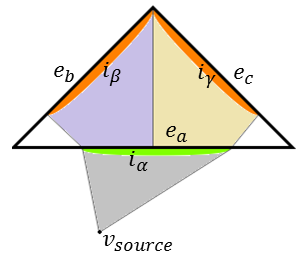
\includegraphics[width=0.75\columnwidth]{images/mmp_algorithm.png}}
	\caption{Propagation scheme of MMP algorithm: interval $i_{\alpha}$ on edge $e_a$ propagate distance pencil paths to adjacent edges $e_b$ and $e_c$ }
	\label{fig:mmp algorithm}
\end{figure}

MMP algorithm creates a geodesic path for "single source and all destination" scheme. The algorithm computes a set of intervals of each edge. An interval represents accessible pencil of lines from its pseudo-source. Each internal also acts as pseudo-source to propagate across faces of the rest of mesh. The algorithm propagates the distance information out from source in a Dijkstra-like fashion which can traceback any positions on mesh back to the source.

The performance of MMP algorithm : They prove a worst case
running time of $O(n^2 \log n)$ when $n$ is number of mesh edges. However in practical calculation, it can achieve on 100K triangles mesh within a few seconds. Also there is approximate version of MMP algorithm proposed by \cite{Surazhsky:2005:FEA:1073204.1073228} that can speed up calculation by trying to merge interval with an adjacent intervals on the same edge before propagation.

\subsection*{Notations}
After calculating exact geodesic distance, each $e_i$ edge that is not boundary edge, has a set of $m$ intervals $I_{e_i}:=\{ i_{e_{i^j}}(f_p,e_p,D) \mid i = 1, ... ,n_v , j = 1,...,m\}$, where $f_p$ represents the face that be crossed by propagation of interval's pseudo-source and $e_p$ represents the edge that has interval's pseudo-source. $D$ represents another informations about geodesic distance of considering interval.

\section{\uppercase{Our Approach}}
\label{sec:our approach}
\noindent Given a triangular 2-manifold mesh $\mathscr{M}$ without any topological information about genus $g$, we adopt the geometry images method \cite{Gu:2002:GI:566654.566589} to define $2g$ cut loop graph for homotopy basis. Instead having cut graph along propagation by geodesic distance criteria, we try to having cut graph in the area where it has same geodesic distance but its pseudo-sources come from different edges.

To define such area, we analyze set of intervals in each edge $e_i$ after calculate geodesic distance \cite{Mitchell:1987:DGP:33367.33372,Surazhsky:2005:FEA:1073204.1073228} as know as MMP algorithm : from a source vertex $v_{s}$. First, we define edges that their intervals have pseudo-sources laid on both side of adjacent faces. However, this case typically can detect few edges and cannot cover all area where the cut graph should be. Second, we define remaining edges that their intervals cannot be a pseudo-source of adjacent edges. we define these two specific characteristic edges into a set of edges $\tilde{E}$. At this point, $\tilde{E}$ contains a lot of dangling edges. Therefore, we eliminate dangling edges from $\tilde{E}$: similar basis as original one.

We ensure that the cut graph has non-separating cycles by considering neighbor edges of $\tilde{E}$. We define a set of neighbor edges $\hat{E}$, 
and candidate cut graph edges be a set of edges $\rho \equiv (\tilde{E} \cup \hat{E})$ and another edges be a set of edges $\acute{E} \equiv (E - \rho)$ . However, $\rho$ may contains contractible cycles too. Therefore, we again need to define non-separating and non-contractible cycles from $\rho$. We follow similar basis from original method by removing an edge adjacent exactly to one triangle. However, we create priority of removing edges in queue as following $\acute{E}$,  $\hat{E}$ and $\tilde{E}$. From this point, we follow the remaining original processes: removing dangling edges and shorten loop.

We explain in details more how to define a set of edge $\tilde{E}$ from two characteristics and how to ensure for generating non-separating and non-contractible cut graph.

\begin{figure}[h!]
	\centering		
	\subfloat[\label{fig:geodesic_both_face}]{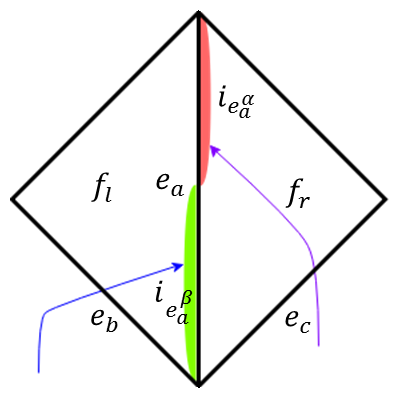
\includegraphics[width=0.45\columnwidth]{images/two_pseudosource.png}}
	\hspace{0.00\columnwidth}
	\subfloat[\label{fig:geodesic_fail_propagte}]{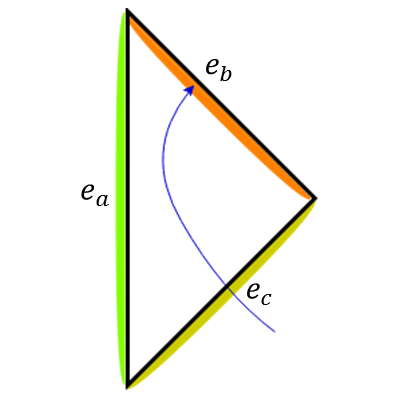
\includegraphics[width=0.45\columnwidth]{images/fail_propagate.png}}
	\hspace{0.00\columnwidth}
	\caption[]{.......}
	\label{fig:fig-two-type-edges}
\end{figure}


\subsection{Edge that pseudo-sources are from both sides}
\label{subsec:pseudo-sources laid on both side of adjacent faces}
The main idea of our approach is to detect the area where geodesic distance's paths are crossing together, similar to wave occlusion. Also, it is the best to detect in edge format since we are creating a cut graph.

First, we detect an edge $e_i$ that its intervals with condition: if there is an interval that $f_p$ is not same as other intervals then we consider $e_i \in \tilde{E}$. From figure \subref*{fig:geodesic_both_face}, we can see clearly that $e_a$ has two intervals $i_{e_{a^\alpha}}$ and $i_{e_{a^\beta}}$ ,which first one has pseudo-source from $f_l$ while second one has pseudo-source from $f_r$. Typically, this kind of edges can be found a fews in mesh (see figure \subref*{fig:edge from two faces}). 

\subsection{Edge that intervals fail to propagate}
Beside edges that be detected in section \ref{subsec:pseudo-sources laid on both side of adjacent faces},  we need to define more edges in cut graph where they are nearby crossing of geodesic distance's paths. 

We detect an edge $e_i$ that its intervals with condition: all intervals have pseudo-sources from same face $f_p$ ($e_p$ can be different). Let opposite face be $f_{\bar{p}}$ and other two edges of $f_{\bar{p}}$ be $e_{\bar{i}_1}$ and $e_{\bar{i}_2}$. We consider both $e_{\bar{i}_1}$ and $e_{\bar{i}_2}$ edges by following condition.
\begin{itemize}
	\item if edge's intervals have pseudo-sources from both sides (section \ref{subsec:pseudo-sources laid on both side of adjacent faces}).
	\item if every edge's intervals have $e_p \neq e_i$.
\end{itemize}

if both edges match one of above condition then we consider $e_i \in \tilde{E}$.

\begin{figure}[h!]
	\centering		
	\subfloat[\label{fig:edge from two faces}]{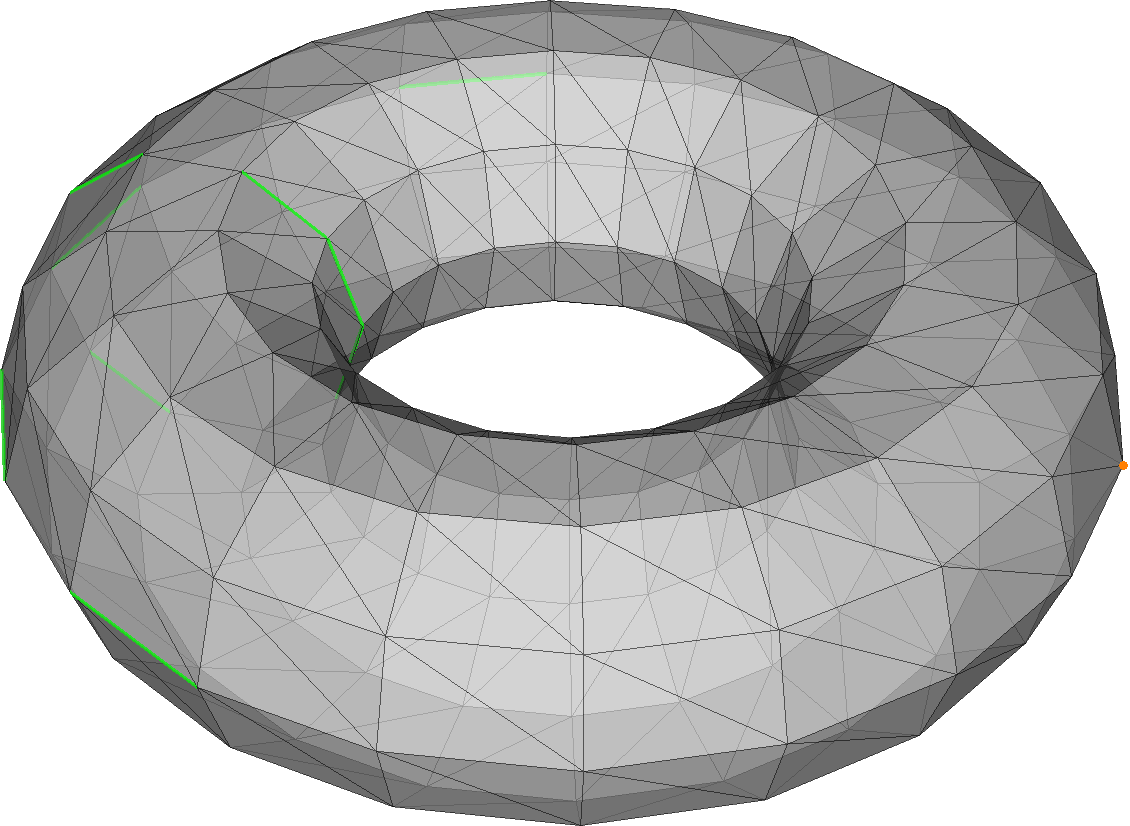
\includegraphics[width=0.45\columnwidth]{images/edge_two_faces.png}}
	\hspace{10pt}
	\subfloat[\label{fig:edge nearby crossing}]{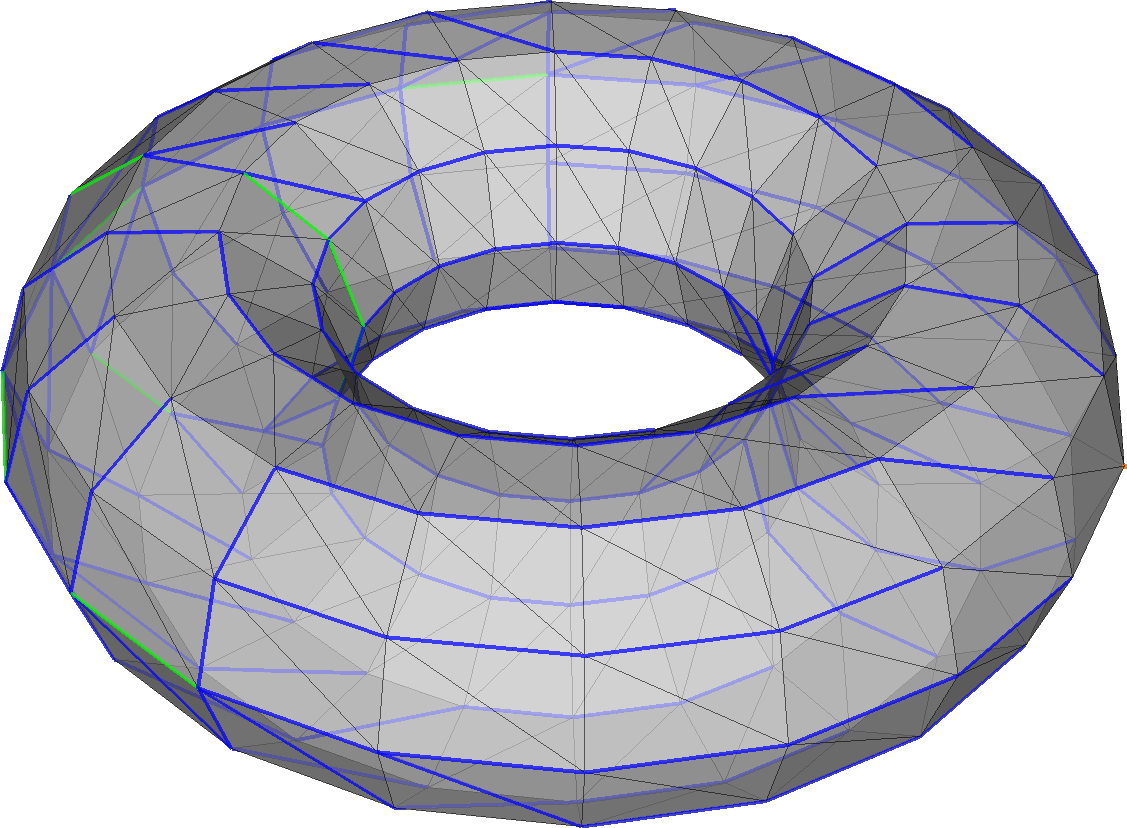
\includegraphics[width=0.45\columnwidth]{images/edge_nearby_crossing.png}}

	\caption[]{.......}
	\label{fig:fig-torus_edges_detected}
\end{figure}

\subsection{Ensure for non-separating and non-contractible cycles}


We classify these remaining edges in the set including their neighbor edges into $\tilde{E}$ to be area where cut graph should be passed through. However, $\tilde{E}$ typically may contains separating or contractible cycles. Therefore, we need to define a valid homotopy cut graph from $\tilde{E}$.
\subsection{Priority Removing-Edge Inside Queue }


\section{\uppercase{Results}}
\label{sec:result}
\section{\uppercase{Conclusions}}
\label{sec:conclusion}

\noindent conclusion....



\section*{\uppercase{Acknowledgements}}
\noindent The images in figure \ref{fig:gim figure} and \ref{fig:fig-original_genus_reducing_process}  are from \cite{Gu:2002:GI:566654.566589} paper and presentation file. This study is supported by JSPS KAKENHI (Grant Number 24300035).


\vfill
\bibliographystyle{apalike}
{\small
\bibliography{genus_cutting}}



\vfill
\end{document}

